Before presenting our analysis of phase delay in software projects, we define our terms, provide an overview of TSP and the sample projects, and describe the data collection process.

\subsection{Definitions}
A \emph{defect} is any change to a product, after its construction, that is necessary to make the product correct.  A typographical error found in review is a defect. If that same defect is discovered while writing the code but before review, it is not considered to be a defect. 

The \emph{cost-to-fix} can be computed in two ways. The first is a direct measure of the actual work time spent in correcting the defect in the product. Direct measurement enables analysis of the variability the cost-to-fix among a category of defects. The second approach measures the total time spent in a defect removal phase and divides by the total defects removed. This provides an average cost-to-fix including overhead of that activity. For example, using method two, a code inspection may require an hour of effort to remove three defects for a 3 defects per hour or to invert the ratio, 1/3 hours per defect. Most of the time, however, is spent locating the defects not actually fixing them. we use the second approach in our analysis.


\subsection{Overview of the Team Software Process}
To empirically test for the phase delay effect, we examined 171 software projects conducted between 2005 and 2014. These projects took place at organizations in many countries and were conducted using  the Team Software Process (TSP$\textsuperscript{SM}$), a software project management approach developed at the Software Engineering Institute (SEI) at Carnegie Mellon University~\cite{tsp00}. TSP is an extension of the Personal Software Process (PSP$\textsuperscript{SM}$) developed at the SEI by Watts Humphrey ~\cite{tsp00}. The data from these TSP projects were collected and stored in the Software Engineering Measured Process Repository (SEMPR) at the SEI. The Software Engineering Institute (SEI) at Carnegie Mellon University explores methods for software process improvement.
 



TSP has guiding principles; the following are relevant to this study:
\begin{itemize}
\item  Sound engineering work does not happen by accident. It must be planned.
\item  Performance of the plans requires realistic commitments of the resources needed to perform the work.
\item  The planned work should frequently be compared to  results to assure plans remain relevant.
\item  People performing the work should be responsible for planning and tracking the work.
\end{itemize}

TSP helps developers by providing a set of measures that can be applied to managing tasks, quality, and schedule. Planning begins by quantifying goals, defining work practices, and estimating size and effort. Developers then use this information to make a detailed short term plan. As the developers perform project work, they use a tool such as the Process Dashboard to collect their time, effort, size, and schedule data. Every week, the team reviews their data to evaluate status, identify actual rates, determine if project goals for schedule, cost, and quality are being met. The team then uses this information to make necessary plan corrections. At the end of the project the coach and team perform a quantitative project post mortem.

Common features of TSP projects include {\em planning}, {\em personal reviews}, {\em peer inspections}, and {\em coaching}.
A TSP {\em coach} helps the team to plan and analyze performance. The coach is the only role authorized to submit project data to the SEI.
Before reviewing data with the teams, therefore before submission, these coaches check the data for obvious errors.

{\em Planning} follows the technique taught in the PSP$\textsuperscript{SM}$. Developers estimate the size of work products and convert this to a total effort using historical rates. Time in specific tasks come from the  process phases and historical percent time in phase distributions. Defects are estimated using historical phase injection rates and phase removal yields. Coaches help the developers to compare estimates against actual results. In this way, developers acquire a more realistic understanding of their work behavior, performance, and schedule status.

{\em Personal review} is a technique taken from the PSP and its use in TSP is unique.  Developers follow a systematic process to remove defects by  examining their own work products using a checklist built from their personal defect profile. This personal review occurs after some product or part of a product is considered to be constructed and before peer reviews or test. 

%PSPSM teaches developers howto continually make and review their personnel estimates
%about their day-to-day tasks, then compare those estimates against the actual development effort.
%In this way, developers can acquire a more realistic understanding of their work behaviour.
  
 
{\em Peer inspection} is a  technique in
traditional software engineering and is often called peer review.
 Basili and Boehm   commented in 2001~\cite{boehm01} 
that peer reviews can catch over half the defects introduced into a system.
Peer inspection can be conducted on any artifact generated anywhere in the software
lifecycle and can quickly be adapted to new kinds of artifacts. TSP peer reviews follow the Fagan style in which the reviewer uses a checklist composed of common team defects prior to a review team meeting. 


\begin{figure}[!t] 
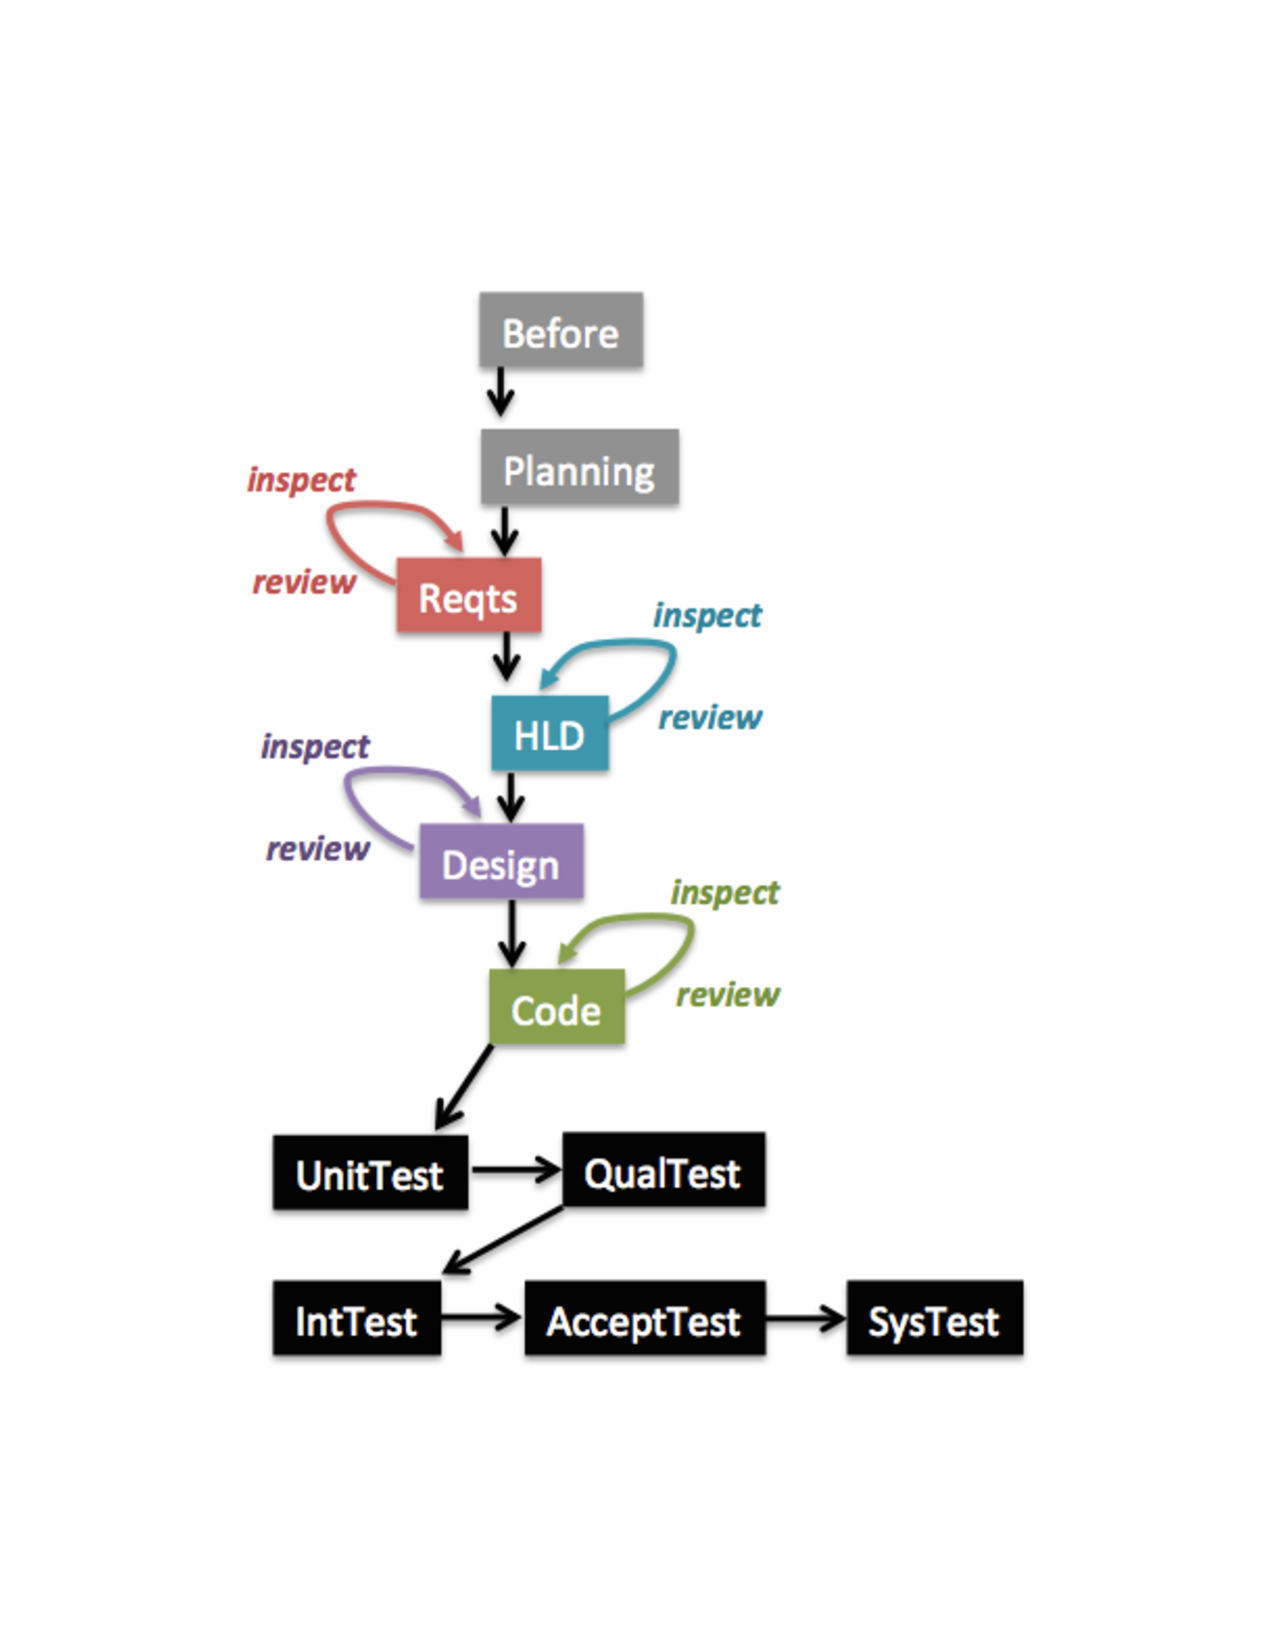
\includegraphics[width=3.5in]{img/waterfall-v3.pdf} 
\caption{Different approaches to software development:  waterfall and agile (bottom left).}
\label{fig:waterfall}
\end{figure}


\subsection{Projects in the Sample}
Since shortly before the year 2000, the SEI has been teaching and coaching TSP teams. One of the authors (Nichols) has been been mentoring software development teams and coaches around the world as they deploy TSP within their organizations since 2006.  The  most recent completions were in 2014.
The projects were mostly small to medium, with a median duration of 46 days and a maximum duration of 90 days in major increments. 
Several projects extended for multiple incremental development cycles. 
Median team size was 7 people, with a maximum of 40. 

Many of the projects were e-commerce web portals or banking systems in the US, South Africa, and Mexico. 
There were  some  medical device projects in  the US, France, Japan, and Germany as well  as a commercial computer-aided design systems, and embedded systems. 

An anonymized version of that data is available in the PROMISE repository\footnote{http://openscience.us/repo}  and,
for confidentiality restrictions, we cannot offer 
further details on these projects.



\subsection{Data Collection Process}
\label{sec:data-collection}

Organizations using TSP agree to provide their project data to the SEI for use in research. In return the SEI agrees    that  data must not be traceable to its source. The data is collected at major project events; launch, interim checkpoints, and at project completion. Data includes project and site  characteristic summaries, surveys of team members, launch presentations, launch outbriefs, and baseline plans, final data from the project, and the project post mortem report.  In practice, this data requirement has only been enforced for the purposes of certifying and reauthorizing TSP coaches who must submit data to maintain their authorization. Coaches are certified by demonstrating competent use of the TSP process with the artifacts and data not by the actual project results.  Of the data submitted, only the data recorded using the Process Dashboard tool has been collected and aggregated for this research. 

To use this data for research and benchmarking,  Nichols first collected the Process Dashboard data from the submission repository then used a tool built by the Process Dashboard developer, David Tuma, 
to gather the project data into a database. Nichols and his colleague Yasutaka Shirai then extracted data into views suitable for analysis. The key views include a project results summary, effort logs, task logs, and defect logs. The data has not yet undergone additional screening. A summary of the data quality issues was reported in a previous work ~\cite{shirai14} (that summary is discussed further in our {\em Validity} section, below).

The tool collected process information about those tasks and defects that we analyze in this work. 
That task data include  work start time, work end time, delta
work time, and interruption time. Software engineers are often
interrupted by meetings, requests for technical help, reporting, and
so forth. These events are recorded, in minutes, as interruption
time. 

 Defect logs include the time and date a defect was discovered, the phase in which that defect was injected, the phase in which it was removed, the time (in minutes) required to find and fix the defect, and the categorical type.

The defect types in the most common defect type standard  in the the SEI TSP data are follows:
\begin{itemize}
\item Environment: design, compile, test, or other support system problems
\item Interface: procedure calls and reference, I/O, user format
\item Data: structure, content
\item Documentation: comments, messages
\item Syntax: spelling, punctuation typos, instruction formats
\item Function: logic, pointers, loops, recursion, computation, function defects  
\item Checking: error messages, inadequate checks
\item Build: change management, library, version control
\item Assignment: package
declaration, duplicate names, scope, limits
\item System: configuration, timing, memory
\end{itemize}


As of November 2014, the SEI TSP database contained data from 212
TSP projects. The projects completed between July 2006 and
November 2014; they included 47 organizations and 843 people. 
The database fact tables
contain 268,726 time logs, 
154,238 task logs,
 47,376 defect logs, 
and 26,534 size logs. 
After selecting defects from the data log and joining the data to the time log table  171 of these projects remained. The excluded projects had no or too few defects to use in this analysis.
 
In this paper, when we report ``time to resolve an
issue,'' we show the difference between the start and end times
of a work session, with any interruption time subtracted (the
difference in times, minus the interruptions). 


%That said, certain semantic features of the SEI TSP data should be noted.
%Firstly, in the current TSP collection tool, 
%fix times are only the developer time for the developer walking through the phases of \fig{waterfall}.
%We are currently tracking the fix time for post-release issues (e.g. those raised during  acceptance test and %later
%product life cycle). So far, in that post-release data,  we have not detected
%a dramatic phase escalation effect (but at this time, we have nothing definitive comment on that matter).%
%
%\bill{somewhere you have one note on \underline{find} and fix times.  for this paper, we need just fix times. %but is there
%anything we need to fret about re \underline{find} times?}
 
 

\subsection{Project Phases}
This paper studies the impact of phase delay on the time required to resolve issues.
The logical phases used in this paper are shown in \fig{waterfall}. Although the representation suggests a waterfall, the phases represent the primary stages through which requirements are developed into working and tested code. That is, all requirements must be stated in some way, implemented in code, integrated, and tested. All real implementations of any size follow a spiral approach with many team performing the work in iterative and/or incremental development cycles.  Within a project increment, multiple features or components may be developed and incremented. TSP is compatible with agile and encourages iterative and incremental development. Nonetheless, the specific strategy and cycle duration is a project decision. TSP does, however, strongly encourage 1) constructing units of sufficient size that measurement is practicable, and 2) separating the construction from appraisal and test activities. This effectively highlights the separation of construction from rework activities and aids the apportionment of defects to those found in appraisal activities (reviews and inspections) and those found through failure (test). The distinct construction activities (requirements, high and detailed design, and code) were chosen to help teams analyze the effectiveness and efficiency of their practices through analysis of the defect phase origin, type, fix effort, and phase of discovery. 

Note that, in that Figure~\ref{fig:waterfall}:
\bi 
\item
Several  phases in which product is created have sub-phases of {\em review} and {\em inspect} to remove defects. TSP uses review, a sub-phase in which individuals perform personal reviews of their work products prior to the peer review, which TSP calls the inspection.
\item Testing is divided into several stages. Developers perform unit test prior to code complete.  After code complete a standard phase is the integration, which combines program units into workable system ready for system test. Integration,  system test, and acceptance test are often performed by a separate group. 
\ei
For these TSP projects, the principles followed are: 
\bi 
%\item Defects should be found before test, that is, test defects should be infrequent.
\item A product should be inspected before used in a subsequent construction phase to minimize  unnecessary rework.
\item To minimize unnecessary rework, a product should be reviewed and inspected prior to use in a subsequent construction phase.
\item A personal review should remove the most common defects before being given to peers for the inspection.
\item Because different categories of test will find different types of defect, and follow in a natural sequence, the tests should be measured separately
\ei 
In summary, the TSP process and measurement have been specifically designed to aid the analysis of defects for use in process improvement. The data are, therefore, uniquely suitable for an analysis of the phase delay effect. 
\subsection{Distinguishing Project Characteristics}
Modern development processes include the core engineering practices of estimation, planning, configuration control, requirements, design, code development, and test. Agile methods address  not only these core practices but also address team organization, individual and team commitments, test and build automation, and implementing iterative and incremental development. TSP uses additional practices associated with high performance ~\cite{jones10} including; project tracking and control, specialization of team members, inspections, static analysis, documentation and training, and reuse. Although the teams in this sample use many typical agile practices, they are also using additional practices. 
